\section{PGStrom}

\href{http://strom.kaigai.gr.jp/}{PGStrom}~--- PostgreSQL расширение, которое позволяет использовать GPU для выполнения некоторых SQL операций. В частности, за счёт привлечения GPU могут быть ускорены такие операции как сравнительный перебор элементов таблиц, агрегирование записей и слияние хэшей. Код для выполнения на стороне GPU генерируется в момент разбора SQL-запроса при помощи специального JIT-компилятора и в дальнейшем выполняется параллельно с другими связанными с текущим запросом операциями, выполняемыми на CPU. Для выполнения заданий на GPU задействован OpenCL. Увеличение производительности операций слияния таблиц (\lstinline!JOIN!) при использовании GPU увеличивается в десятки раз.

\begin{figure}[ht!]
  \center{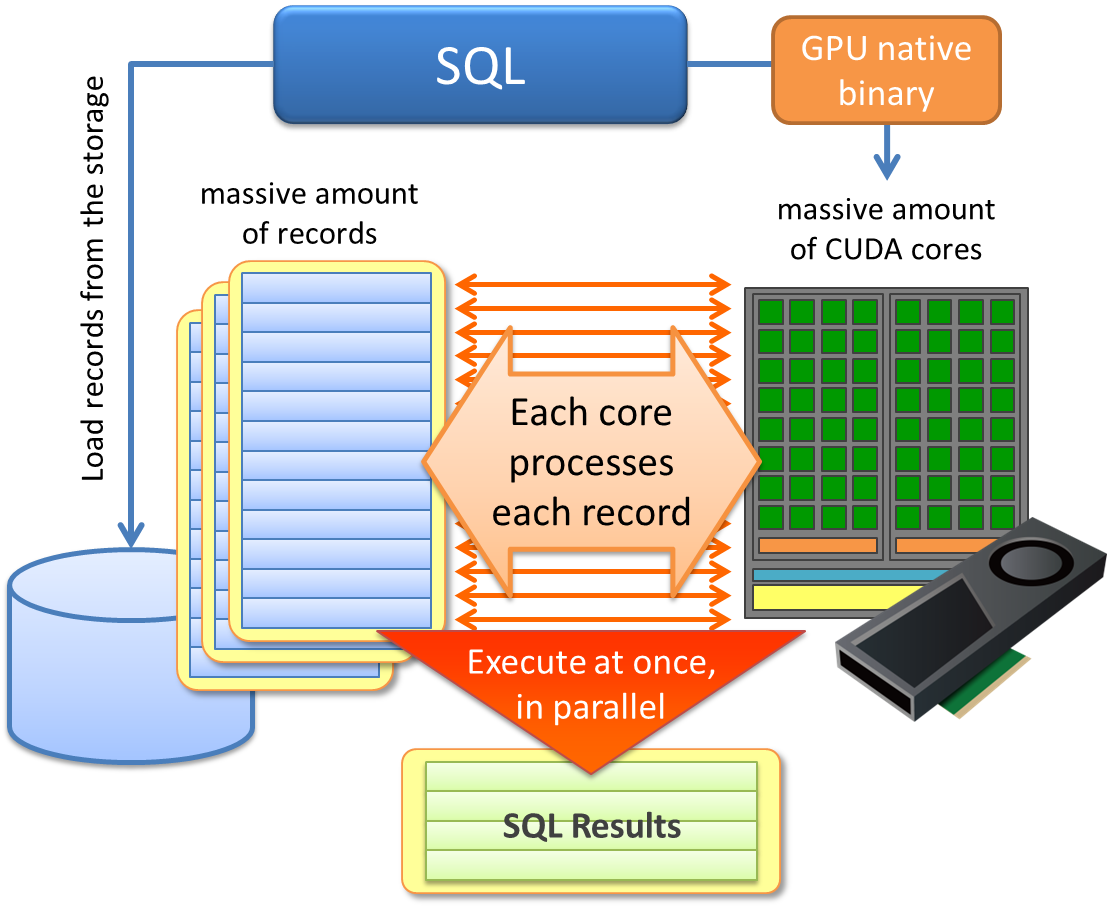
\includegraphics[width=1\textwidth]{pgstrom_gpu_power.pdf}}
  \caption{PGStrom}
  \label{fig:pgstrom1}
\end{figure}

Областью применения PG-Strom являются огромные отчеты с использованием агрегации и объединения таблиц. Эти рабочие нагрузки чаще используются в пакетной обработке данных для \href{https://ru.wikipedia.org/wiki/OLAP}{OLAP} систем.
